% 原文PDF54--74頁（本文32--52頁）、第2章導入および2.1--2.5。
\sectionlink{共形場理論}\label{ch:2}

この章では、演算子積展開、共形不変性、Virasoro 代数、頂点演算子など、世界面の場の量子論から必要となるいくつかの考え方と手法を展開する。中心となるのは、平坦な二次元における共形不変な場の理論である。次章で見るように、これは弦の世界面の局所対称性を固定した後に残るものである。

\subsectionlink{二次元の質量のないスカラー}\label{sec:2.1}

まず、二次元の $D$ 個の自由スカラー場 $X^\mu(\sigma^1,\sigma^2)$ の例から始める。弦理論への応用を見越して、この二次元を世界面と呼ぶ。作用は
\begin{equation}
S=\frac{1}{4\pi\alpha'}\int d^2\sigma\,
\left(\partial_1X^\mu\partial_1X_\mu+\partial_2X^\mu\partial_2X_\mu\right)
\tag{2.1.1}\label{eq:2.1.1}
\end{equation}
である。これは、世界面計量 $\gamma_{ab}$ を符号 $(+,+)$ の平坦な Euclid 計量 $\delta_{ab}$ で置き換えたことを除けば、Polyakov 作用\hyperref[eq:1.2.13]{(1.2.13)}である。作用全体の符号の変化は、Euclid の規約(A.1.31)による。後で見るように、弦の計算の大部分は Euclid 世界面上で行われる。少なくとも平坦な計量の場合、Euclid 振幅と Minkowski 振幅の関係は、付録で説明する標準的な解析接続によって与えられる。実際、この章の結果は Minkowski 世界面にも同様に適用され、最初の七つの節のすべての式は、$\sigma^2$ を $i\sigma^0$ に置き換えても意味をもつ。添字 $\mu$ に対しては、引き続き平坦な Minkowski 計量を用いる。

作用\hyperref[eq:2.1.1]{(2.1.1)}を正準量子化し、スペクトルや真空期待値などを求めることは容易である。第1章で光円錐ゲージに移った後に行ったのは、本質的にこれであった。ここでは少し違う道筋をとり、運動方程式、演算子積、Ward 恒等式、共形不変性などのさまざまな局所的性質を先に展開してから、スペクトルへと進む。経路積分の形式を用いるのが効率的であり、付録でこれを復習している。経路積分表示は、主として以下で定義する演算子方程式を導くために用いる。これらは Hilbert 空間の形式でも導出できる。

複素座標
\begin{equation}
z=\sigma^1+i\sigma^2,\qquad \bar z=\sigma^1-i\sigma^2
\tag{2.1.2}\label{eq:2.1.2}
\end{equation}
を採用すると非常に便利である。$z$ などの簡単な変数の複素共役には上線を用い、より長い式の複素共役には星印を用いる。また、
\begin{equation}
\partial_z=\frac12(\partial_1-i\partial_2),\qquad
\partial_{\bar z}=\frac12(\partial_1+i\partial_2)
\tag{2.1.3}\label{eq:2.1.3}
\end{equation}
と定義する。これらの微分は
\begin{equation}
\partial_z z=1,\qquad \partial_z\bar z=0,\qquad
\partial_{\bar z}z=0,\qquad \partial_{\bar z}\bar z=1
\tag{2.1.4}\label{eq:2.1.4}
\end{equation}
という性質をもつ。曖昧さがない場合、$\partial_z$ を $\partial$、$\partial_{\bar z}$ を $\bar\partial$ と略記するのが慣例である。一般のベクトル $v^a$ に対しても、同様に
\begin{equation}
\begin{gathered}
v^z=v^1+iv^2,\qquad v^{\bar z}=v^1-iv^2,\\
v_z=\frac12(v^1-iv^2),\qquad
v_{\bar z}=\frac12(v^1+iv^2)
\end{gathered}
\tag{2.1.5}\label{eq:2.1.5}
\end{equation}
と定義する。添字 $1,2$ に対しては計量は単位行列であり、上付きと下付きを区別しない。一方、複素添字の上げ下げには
\begin{equation}
\begin{gathered}
g_{z\bar z}=g_{\bar z z}=\frac12,\qquad
g_{zz}=g_{\bar z\bar z}=0,\\
g^{z\bar z}=g^{\bar z z}=2,\qquad
g^{zz}=g^{\bar z\bar z}=0
\end{gathered}
\tag{2.1.6}\label{eq:2.1.6}
\end{equation}
を用いる。また、
\begin{equation}
d^2z=2\,d\sigma^1d\sigma^2
\tag{2.1.7}\label{eq:2.1.7}
\end{equation}
であることにも注意しよう。この因子2は Jacobian に由来する。\footnote[1]{これは、$d^2z$ を $d\sigma^1d\sigma^2$ と定義する多くの文献とは異なる。それに対応して、それらの文献では $\delta^2(z,\bar z)$ の定義から $\tfrac12$ が省かれている。}
したがって、$d^2z\,|\det g|^{1/2}=d\sigma^1d\sigma^2$ である。
\begin{equation}
\int d^2z\,\delta^2(z,\bar z)=1
\tag{2.1.8}\label{eq:2.1.8}
\end{equation}
と定義するので、$\delta^2(z,\bar z)=\tfrac12\delta(\sigma^1)\delta(\sigma^2)$ となる。もう一つの有用な結果は、複素座標における発散定理
\begin{equation}
\int_Rd^2z\,(\partial_zv^z+\partial_{\bar z}v^{\bar z})
=i\oint_{\partial R}(v^z\,d\bar z-v^{\bar z}\,dz)
\tag{2.1.9}\label{eq:2.1.9}
\end{equation}
である。ここで、線積分は領域 $R$ の周りを反時計回りに巡る。

この記法では、作用は
\begin{equation}
S=\frac{1}{2\pi\alpha'}\int d^2z\,\partial X^\mu\bar\partial X_\mu
\tag{2.1.10}\label{eq:2.1.10}
\end{equation}
となり、古典的な運動方程式は
\begin{equation}
\partial\bar\partial X^\mu(z,\bar z)=0
\tag{2.1.11}\label{eq:2.1.11}
\end{equation}
となる。$z$ の値が $\bar z$ の値を決めるので、$X^\mu(z,\bar z)$ という記法は冗長に見えるかもしれない。しかし、$f(z)$ という記法を、運動方程式によって $z$ の解析的、すなわち正則な関数となる場のために取っておくと便利である。運動方程式を
\begin{equation}
\partial(\bar\partial X^\mu)=\bar\partial(\partial X^\mu)=0
\tag{2.1.12}\label{eq:2.1.12}
\end{equation}
と書けば、$\partial X^\mu$ は正則、$\bar\partial X^\mu$ は反正則（$\bar z$ に関して正則）であることが従う。このため、$\partial X^\mu(z)$、$\bar\partial X^\mu(\bar z)$ と表記する。

Minkowski への接続 $\sigma^2=i\sigma^0$ の下で、正則な場は $\sigma^0-\sigma^1$ だけの関数となり、反正則な場は $\sigma^0+\sigma^1$ だけの関数となる。したがって、次を同義語として用いる。
\begin{align}
\text{正則}&=\text{左向き},\tag{2.1.13a}\label{eq:2.1.13a}\\
\text{反正則}&=\text{右向き}.\tag{2.1.13b}\label{eq:2.1.13b}
\end{align}
この用語は、文献との一致をできるだけ大きくするように選んだものである。ただし、これを文字どおり成立させるためには、$\sigma^1$ が右から左に向かって増加するように図を描く必要がある。初めのうちは Euclid の用語を多く用い、時空の物理をより多く論じるようになるにつれて、Minkowski の用語へ移っていくことにする。

期待値は経路積分によって定義する。
\begin{equation}
\langle\mathcal F[X]\rangle=\int[dX]\,\exp(-S)\mathcal F[X].
\tag{2.1.14}\label{eq:2.1.14}
\end{equation}
ここで $\mathcal F[X]$ は、局所演算子の積など、$X$ の任意の汎関数である。$X^0$ についての経路積分は符号が逆の Gauss 積分なので、解析接続 $X^0\to-iX^D$ によって定義されると理解すべきである。読者はこの点に気を取られる必要はない。次章でさらに議論する。$\langle\mathcal F[X]\rangle$ を $\langle1\rangle$ で割って規格化することはしない。

全微分の経路積分はゼロである。これは、無限個の通常の積分の極限とみなせる普通のボソンの経路積分についても、Grassmann 変数を用いるような、より形式的な経路積分についても正しい。したがって、
\begin{equation}
\begin{aligned}
0&=\int[dX]\,\frac{\delta}{\delta X_\mu(z,\bar z)}\exp(-S)\\
&=-\int[dX]\,\exp(-S)\frac{\delta S}{\delta X_\mu(z,\bar z)}\\
&=-\left\langle\frac{\delta S}{\delta X_\mu(z,\bar z)}\right\rangle\\
&=\frac{1}{\pi\alpha'}\left\langle\partial\bar\partial X^\mu(z,\bar z)\right\rangle.
\end{aligned}
\tag{2.1.15}\label{eq:2.1.15}
\end{equation}
経路積分に任意の追加の挿入「$\cdots$」があっても、それらのいずれも $z$ に置かれていなければ、同じ計算が成り立つ。したがって、
\begin{equation}
\left\langle\partial\bar\partial X^\mu(z,\bar z)\cdots\right\rangle=0.
\tag{2.1.16}\label{eq:2.1.16}
\end{equation}
これらの追加の挿入は、任意の始状態と終状態を準備するものとみなせる（境界条件を用いても同じことができる）。ゆえに、経路積分における主張\hyperref[eq:2.1.16]{(2.1.16)}は、Hilbert 空間の形式において、
\begin{equation}
\partial\bar\partial\widehat X^\mu(z,\bar z)=0
\tag{2.1.17}\label{eq:2.1.17}
\end{equation}
が演算子 $\widehat X^\mu(z,\bar z)$ のすべての行列要素について成り立つという主張と同じである。そこで、\hyperref[eq:2.1.16]{(2.1.16)}の意味で成り立つ関係を演算子方程式と呼ぶ。\hyperref[eq:2.1.17]{(2.1.17)}という主張は、古典的な運動方程式が演算子方程式に移されるという Ehrenfest の定理である。

経路積分\hyperref[eq:2.1.16]{(2.1.16)}における記号「$\cdots$」は、暗黙のうちに $z$ から離れた位置の挿入を表している。しかし、$z$ と一致する可能性のある挿入がある場合も考えると興味深い。
\begin{equation}
\begin{aligned}
0={}&\int[dX]\,\frac{\delta}{\delta X_\mu(z,\bar z)}
\left[\exp(-S)X^\nu(z',\bar z')\right]\\
={}&\int[dX]\,\exp(-S)\left[
\eta^{\mu\nu}\delta^2(z-z',\bar z-\bar z')
+\frac{1}{\pi\alpha'}\partial_z\partial_{\bar z}X^\mu(z,\bar z)
X^\nu(z',\bar z')\right]\\
={}&\eta^{\mu\nu}\left\langle\delta^2(z-z',\bar z-\bar z')\right\rangle
+\frac{1}{\pi\alpha'}\partial_z\partial_{\bar z}
\left\langle X^\mu(z,\bar z)X^\nu(z',\bar z')\right\rangle.
\end{aligned}
\tag{2.1.18}\label{eq:2.1.18}
\end{equation}
つまり、運動方程式は一致点を除いて成り立つ。ここでも、経路積分に任意の追加の挿入「$\cdots$」があっても、その追加の場のいずれも $(z,\bar z)$ または $(z',\bar z')$ に置かれていなければ、同じ議論が成り立つ。
\begin{equation}
\begin{aligned}
&\frac{1}{\pi\alpha'}\partial_z\partial_{\bar z}
\left\langle X^\mu(z,\bar z)X^\nu(z',\bar z')\cdots\right\rangle\\
&\hspace{2em}=-\eta^{\mu\nu}
\left\langle\delta^2(z-z',\bar z-\bar z')\cdots\right\rangle.
\end{aligned}
\tag{2.1.19}\label{eq:2.1.19}
\end{equation}
したがって、
\begin{equation}
\frac{1}{\pi\alpha'}\partial_z\partial_{\bar z}
X^\mu(z,\bar z)X^\nu(z',\bar z')
=-\eta^{\mu\nu}\delta^2(z-z',\bar z-\bar z')
\tag{2.1.20}\label{eq:2.1.20}
\end{equation}
が演算子方程式として成り立つ。Hilbert 空間の形式では、経路積分中の積は時間順序積となり、デルタ関数は微分が時間順序に作用することから生じる。この関係は付録でさらに展開する。

自由場の理論では、正規順序という操作を導入すると便利である。$:\mathcal A:$ と表す正規順序化された演算子を、次のように定義する。
\begin{align}
:X^\mu(z,\bar z):&=X^\mu(z,\bar z),
\tag{2.1.21a}\label{eq:2.1.21a}\\
:X^\mu(z_1,\bar z_1)X^\nu(z_2,\bar z_2):
&=X^\mu(z_1,\bar z_1)X^\nu(z_2,\bar z_2)
+\frac{\alpha'}2\eta^{\mu\nu}\ln|z_{12}|^2.
\tag{2.1.21b}\label{eq:2.1.21b}
\end{align}
ここで
\begin{equation}
z_{ij}=z_i-z_j
\tag{2.1.22}\label{eq:2.1.22}
\end{equation}
である。読者は、上昇演算子と下降演算子によって定義される正規順序を知っているかもしれない。この二つの定義は後で関係づける。この定義の要点は、
\begin{equation}
\partial_1\bar\partial_1:X^\mu(z_1,\bar z_1)X^\nu(z_2,\bar z_2):=0
\tag{2.1.23}\label{eq:2.1.23}
\end{equation}
という性質である。これは、演算子方程式\hyperref[eq:2.1.20]{(2.1.20)}と微分方程式
\begin{equation}
\partial\bar\partial\ln|z|^2=2\pi\delta^2(z,\bar z)
\tag{2.1.24}\label{eq:2.1.24}
\end{equation}
から従う。$z\ne0$ では $\ln|z|^2=\ln z+\ln\bar z$ であるため、式\hyperref[eq:2.1.24]{(2.1.24)}は明らかである。デルタ関数の規格化も、式\hyperref[eq:2.1.9]{(2.1.9)}を用いて両辺を積分すれば容易に確認できる。

\subsectionlink{演算子積展開}\label{sec:2.2}

弦の摂動論で関心の対象となる基本的な量は、局所演算子の積の経路積分期待値
\begin{equation}
\left\langle\mathcal A_{i_1}(z_1,\bar z_1)
\mathcal A_{i_2}(z_2,\bar z_2)\cdots
\mathcal A_{i_n}(z_n,\bar z_n)\right\rangle
\tag{2.2.1}\label{eq:2.2.1}
\end{equation}
である。ここで $\mathcal A_i$ は、局所演算子の集合のある基底である。二つの演算子を互いに近づける極限で、この期待値がどのように振る舞うかを理解することが、とくに重要である。この極限を系統的に記述する道具が、図\hyperref[fig:2.1]{2.1}に示す演算子積展開（OPE）である。これは、互いに近い二つの局所演算子の積が、局所演算子の和によって任意の精度まで近似できるというものである。
\begin{equation}
\mathcal A_i(\sigma_1)\mathcal A_j(\sigma_2)
=\sum_kc^k{}_{ij}(\sigma_1-\sigma_2)\mathcal A_k(\sigma_2).
\tag{2.2.2}\label{eq:2.2.2}
\end{equation}
これも演算子としての主張であり、$\sigma_1$ と $\sigma_2$ の間隔が、ほかのどの演算子までの距離に比べても小さい限り、一般の期待値の内部で
\begin{equation}
\left\langle\mathcal A_i(\sigma_1)\mathcal A_j(\sigma_2)\cdots\right\rangle
=\sum_kc^k{}_{ij}(\sigma_1-\sigma_2)
\left\langle\mathcal A_k(\sigma_2)\cdots\right\rangle
\tag{2.2.3}\label{eq:2.2.3}
\end{equation}
が成り立つことを意味する。間隔への依存性を支配する係数関数 $c^k{}_{ij}(\sigma_1-\sigma_2)$ は $i,j,k$ に依存するが、期待値の中のほかの演算子には依存しない。後者への依存性は、式\hyperref[eq:2.2.3]{(2.2.3)}の右辺の期待値を通じてのみ現れる。各項は慣例として、$\sigma_1\to\sigma_2$ の極限で大きさが減少する順に並べる。これは通常の Taylor 級数に類似しているが、係数関数が単純なべきである必要はなく、最も単純な例でさえ見るように、実際には $\sigma_1\to\sigma_2$ で特異になりうる点が異なる。Taylor 級数が微積分で中心的な役割を果たすのと同様に、OPE は場の量子論で中心的な役割を果たす。

\begin{figure}[htbp]
\centering
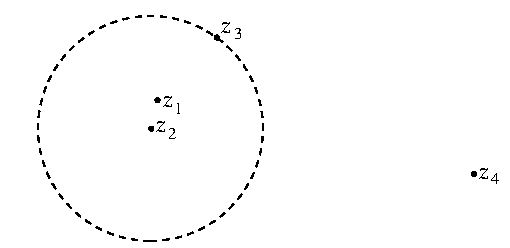
\includegraphics[width=0.8\linewidth]{figures/fig_2_1.pdf}
\caption{四つの局所演算子の積の期待値。OPE は、$z_1$ と $z_2$ の二つの演算子を $z_2$ の一つの演算子で置き換えた級数として、$z_1\to z_2$ での漸近的振る舞いを与える。収束半径は、最も近いほかの演算子までの距離であり、破線の円で示してある。}
\label{fig:2.1}
\end{figure}

ここでは、自由場の理論の特別な性質を用いて、$X^\mu$ 理論の OPE を導く。2.9節では、任意の共形不変な場の理論について導出する。

正規順序積が、素朴な運動方程式を満たすことを見た。式\hyperref[eq:2.1.23]{(2.1.23)}は、演算子積が $(z_1,\bar z_1)$ の調和関数であることを述べている。複素関数論の簡単な結果によれば、調和関数は局所的に、正則関数と反正則関数の和である。とくに、これは $z_1\to z_2$ で非特異であり、$z_{12}$ と $\bar z_{12}$ について自由に Taylor 展開できることを意味する。したがって、
\begin{equation}
\begin{aligned}
X^\mu(z_1,\bar z_1)X^\nu(z_2,\bar z_2)
={}&-\frac{\alpha'}2\eta^{\mu\nu}\ln|z_{12}|^2
+:X^\nu X^\mu(z_2,\bar z_2):\\
&+\sum_{k=1}^\infty\frac1{k!}\Bigl[
(z_{12})^k:X^\nu\partial^kX^\mu(z_2,\bar z_2):\\
&\hspace{8em}
+(\bar z_{12})^k:X^\nu\bar\partial^kX^\mu(z_2,\bar z_2):\Bigr].
\end{aligned}
\tag{2.2.4}\label{eq:2.2.4}
\end{equation}
混合した $\partial\bar\partial$ 微分を含む項は、運動方程式によって消える。この式とほかの多くの式は、$\alpha'=2$ とする単位で簡単になり、これが文献で最も一般的な規約である。しかし、ほかにもいくつかの規約が使われるため、$\alpha'$ を明示しておくと便利である。たとえば、開弦理論では $\alpha'=\tfrac12$ とすると式が簡単になる。

式\hyperref[eq:2.2.4]{(2.2.4)}は OPE の形をしている。その導出のもととなった運動方程式\hyperref[eq:2.1.23]{(2.1.23)}と同様に、これは演算子としての主張である。積 $X^\mu(z_1,\bar z_1)X^\nu(z_2,\bar z_2)$ に、ほかの点の場を掛けたものを含む任意の期待値に対して、$z_1\to z_2$ での振る舞いを無限級数として与える。各項は、$z_{12}$ および／または $\bar z_{12}$ の既知の関数と、二つの演算子を局所演算子で置き換えた期待値との積である。

OPE は通常、漸近展開として用いられ、最初の数項が小さい間隔での支配的な振る舞いを与える。本書の応用の大部分もこの種のものであり、しばしば OPE を、明示した特異項と、具体的に書かない非特異な残余との和として記す。「$=$」の代わりに「$\sim$」を用いたときは、「非特異な項を除いて等しい」という意味である。実際には、共形不変な場の理論では OPE は収束する。このことは、ある種の応用において非常に重要であり、係数関数から理論全体を再構成することを可能にする。一例として、自由場の OPE \hyperref[eq:2.2.4]{(2.2.4)}の任意の期待値における収束半径は、経路積分内の最も近いほかの挿入までの距離に等しい。演算子積は、演算子の位置を除いて調和関数であり、とくに図\hyperref[fig:2.1]{2.1}の破線の円の内部で調和である。そのため、複素関数論の標準的な議論によって収束を示すことができる。

OPE \hyperref[eq:2.2.4]{(2.2.4)}の右辺のさまざまな演算子には、同じ点における場の積が含まれている。場の量子論では、通常このような積は発散し、適切にカットオフを入れて繰り込まねばならないが、ここでは正規順序によって明確に定義される。正規順序は、自由場の理論で複合演算子を定義する便利な方法である。相互作用する場の理論の大部分では、相互作用頂点が複合演算子に近づいたり、互いに近づいたりすることによる追加の発散があるため、ほとんど役に立たない。しかし、われわれが関心をもつ場の理論の多くは自由であり、ほかの多くも自由場の理論と関係づけられる。したがって、正規順序をもう少し展開しておく価値がある。

任意の数の場に対する正規順序の定義は、次のように再帰的に与えられる。
\begin{equation}
\begin{aligned}
&:X^{\mu_1}(z_1,\bar z_1)\cdots X^{\mu_n}(z_n,\bar z_n):\\
&\qquad=X^{\mu_1}(z_1,\bar z_1)\cdots X^{\mu_n}(z_n,\bar z_n)
+\sum\text{減算項}.
\end{aligned}
\tag{2.2.5}\label{eq:2.2.5}
\end{equation}
ここで和は、積から一組、二組、あるいはそれ以上の場の対を選ぶすべての方法にわたり、それぞれの対を $\tfrac12\alpha'\eta^{\mu_i\mu_j}\ln|z_{ij}|^2$ で置き換える。たとえば、
\begin{equation}
\begin{aligned}
&:X^{\mu_1}(z_1,\bar z_1)X^{\mu_2}(z_2,\bar z_2)X^{\mu_3}(z_3,\bar z_3):\\
&\quad=X^{\mu_1}(z_1,\bar z_1)X^{\mu_2}(z_2,\bar z_2)X^{\mu_3}(z_3,\bar z_3)\\
&\qquad+\left(\frac{\alpha'}2\eta^{\mu_1\mu_2}\ln|z_{12}|^2
X^{\mu_3}(z_3,\bar z_3)+\text{二つの置換項}\right).
\end{aligned}
\tag{2.2.6}\label{eq:2.2.6}
\end{equation}
定義\hyperref[eq:2.2.5]{(2.2.5)}が、正規順序積は素朴な運動方程式を満たすという望ましい性質を保つことの証明は、読者に委ねる。

この定義は簡潔に
\begin{equation}
:\mathcal F:
=\exp\left(\frac{\alpha'}4\int d^2z_1d^2z_2\,
\ln|z_{12}|^2\,
\frac{\delta}{\delta X^\mu(z_1,\bar z_1)}
\frac{\delta}{\delta X_\mu(z_2,\bar z_2)}\right)\mathcal F
\tag{2.2.7}\label{eq:2.2.7}
\end{equation}
とまとめられる。ここで $\mathcal F$ は $X$ の任意の汎関数である。これは式\hyperref[eq:2.2.5]{(2.2.5)}と等価である。指数の中の二重微分が場の各対を縮約し、指数関数が任意の数の対について和をとる。その際、階乗が微分の作用の仕方の数を打ち消す。この形式的な表式の使い方の一例として、両辺に逆の指数関数を作用させると、
\begin{equation}
\begin{aligned}
\mathcal F
&=\exp\left(-\frac{\alpha'}4\int d^2z_1d^2z_2\,
\ln|z_{12}|^2\,
\frac{\delta}{\delta X^\mu(z_1,\bar z_1)}
\frac{\delta}{\delta X_\mu(z_2,\bar z_2)}\right):\mathcal F:\\
&=:\mathcal F:+\sum\text{縮約項}
\end{aligned}
\tag{2.2.8}\label{eq:2.2.8}
\end{equation}
を得る。ここで縮約は減算の逆であり、$:\mathcal F:$ から一組、二組、あるいはそれ以上の場の対を選ぶすべての方法について和をとり、各対を $-\tfrac12\alpha'\eta^{\mu_i\mu_j}\ln|z_{ij}|^2$ で置き換える。

任意の二つの演算子の OPE は、$X$ の任意の汎関数 $\mathcal F,\mathcal G$ に対する
\begin{equation}
:\mathcal F:\,:\mathcal G:
=:\mathcal F\mathcal G:+\sum\text{交差縮約項}
\tag{2.2.9}\label{eq:2.2.9}
\end{equation}
から生成できる。今度の和は、$\mathcal F$ 中の一つの場と $\mathcal G$ 中の一つの場を対にして縮約するすべての方法にわたる。これはまた、
\begin{equation}
:\mathcal F:\,:\mathcal G:
=\exp\left(-\frac{\alpha'}2\int d^2z_1d^2z_2\,\ln|z_{12}|^2\,
\frac{\delta}{\delta X_{\mathcal F}^{\mu}(z_1,\bar z_1)}
\frac{\delta}{\delta X_{\mathcal G\mu}(z_2,\bar z_2)}\right)
:\mathcal F\mathcal G:
\tag{2.2.10}\label{eq:2.2.10}
\end{equation}
とも書ける。ここで汎関数微分は、それぞれ $\mathcal F$ または $\mathcal G$ 中の場にだけ作用する。これは式\hyperref[eq:2.2.7]{(2.2.7)}から容易に従う。

一例として、
\begin{equation}
\begin{aligned}
&:\partial X^\mu(z)\partial X_\mu(z):
:\partial'X^\nu(z')\partial'X_\nu(z'):\\
&\quad=:\partial X^\mu(z)\partial X_\mu(z)
\partial'X^\nu(z')\partial'X_\nu(z'):\\
&\qquad-4\cdot\frac{\alpha'}2
\bigl(\partial\partial'\ln|z-z'|^2\bigr)
:\partial X^\mu(z)\partial'X_\mu(z'):\\
&\qquad+2\cdot\eta^\mu{}_\mu
\left(-\frac{\alpha'}2\partial\partial'\ln|z-z'|^2\right)^2\\
&\quad\sim\frac{D\alpha'^2}{2(z-z')^4}
-\frac{2\alpha'}{(z-z')^2}:\partial'X^\mu(z')\partial'X_\mu(z'):\\
&\qquad-\frac{2\alpha'}{z-z'}
:\partial'^2X^\mu(z')\partial'X_\mu(z'):.
\end{aligned}
\tag{2.2.11}\label{eq:2.2.11}
\end{equation}
等号の右辺の第2項は、一組の対を作る四つの方法から生じ、第3項は、二組の対を作る二つの方法から生じる。最後の式では、正規順序の内部で Taylor 展開してすべてを $z'$ の局所演算子で表し、最も特異な項を先頭に置くことで、OPE を標準形にしている。

もう一つの重要な例は
\begin{equation}
\mathcal F=e^{ik_1\cdot X(z,\bar z)},\qquad
\mathcal G=e^{ik_2\cdot X(0,0)}
\tag{2.2.12}\label{eq:2.2.12}
\end{equation}
である。変分 $\delta/\delta X_{\mathcal F}^\mu$ と
$\delta/\delta X_{\mathcal G}^\mu$ は、それぞれ $ik_{1\mu}$ と $ik_{2\mu}$ の因子を与える。したがって、一般的な結果\hyperref[eq:2.2.10]{(2.2.10)}は
\begin{equation}
\begin{aligned}
:e^{ik_1\cdot X(z,\bar z)}:\,:e^{ik_2\cdot X(0,0)}:
&=\exp\left(\frac{\alpha'}2k_1\cdot k_2\ln|z|^2\right)
:e^{ik_1\cdot X(z,\bar z)}e^{ik_2\cdot X(0,0)}:\\
&=|z|^{\alpha'k_1\cdot k_2}
:e^{ik_1\cdot X(z,\bar z)}e^{ik_2\cdot X(0,0)}:
\end{aligned}
\tag{2.2.13}\label{eq:2.2.13}
\end{equation}
となる。OPE を導くには、正規順序の内部で Taylor 展開して、
\begin{equation}
:e^{ik_1\cdot X(z,\bar z)}:\,:e^{ik_2\cdot X(0,0)}:
=|z|^{\alpha'k_1\cdot k_2}
:e^{i(k_1+k_2)\cdot X(0,0)}[1+O(z,\bar z)]:
\tag{2.2.14}\label{eq:2.2.14}
\end{equation}
を得ればよい。演習では、正規順序と自由場の OPE をさらに練習する。

OPE \hyperref[eq:2.2.2]{(2.2.2)}、\hyperref[eq:2.2.4]{(2.2.4)}などは、後者の点の周りで展開することで、$\sigma_1,\sigma_2$ に関して非対称に書かれていることに注意しよう。右辺を $(\sigma_1+\sigma_2)/2$ の周りで Taylor 展開すれば、対称な形にもできる。対称な形の係数関数は、二つの演算子の交換に対して単純に振る舞う。
\begin{equation}
c^k{}_{ij}(\sigma_1-\sigma_2)_{\mathrm{sym}}
=\pm c^k{}_{ji}(\sigma_2-\sigma_1)_{\mathrm{sym}}.
\tag{2.2.15}\label{eq:2.2.15}
\end{equation}
ここで、$\mathcal A_i$ と $\mathcal A_j$ がともに反交換する場合には、負号が現れる。計算には通常、非対称な形の方が便利であるため、係数関数の対称性が必要な場合には、対称な形でそれを求めてから、非対称な形に変換すればよい。

\subsectionlink{Ward 恒等式と Noether の定理}\label{sec:2.3}

世界面の対称性が弦理論で重要な役割を果たすことは、もちろんである。この節ではまず、場の理論における対称性の一般的な帰結をいくつか導く。

$d$ 次元時空における、作用 $S[\phi]$ をもつ一般の場の理論を考える。$\phi_\alpha(\sigma)$ は一般の場を表す。対称変換
\begin{equation}
\phi'_\alpha(\sigma)=\phi_\alpha(\sigma)+\delta\phi_\alpha(\sigma)
\tag{2.3.1}\label{eq:2.3.1}
\end{equation}
があり、$\delta\phi_\alpha$ は無限小パラメータ $\epsilon$ に比例するものとする。経路積分の測度と重み $\exp(-S)$ の積は不変である。
\begin{equation}
[d\phi']\exp\bigl(-S[\phi']\bigr)
=[d\phi]\exp\bigl(-S[\phi]\bigr).
\tag{2.3.2}\label{eq:2.3.2}
\end{equation}

場の理論の連続対称性は、保存カレントの存在（Noether の定理）と、カレントの演算子積を制約する Ward 恒等式を意味する。これらの結果を導くため、変数変換
\begin{equation}
\phi'_\alpha(\sigma)=\phi_\alpha(\sigma)
+\rho(\sigma)\delta\phi_\alpha(\sigma)
\tag{2.3.3}\label{eq:2.3.3}
\end{equation}
を考える。任意関数 $\rho(\sigma)$ を含めることで変換則を変更しているので、これは対称変換ではない。もし $\rho$ が定数なら、経路積分測度と $\exp(-S)$ の積は不変であるため、その変分は勾配 $\partial_a\rho$ に比例しなければならない。
\begin{equation}
\begin{aligned}
&[d\phi']\exp\bigl(-S[\phi']\bigr)\\
&\quad=[d\phi]\exp\bigl(-S[\phi]\bigr)
\left[1+\frac{i\epsilon}{2\pi}\int d^d\sigma\,g^{1/2}
j^a(\sigma)\partial_a\rho(\sigma)+O(\epsilon^2)\right].
\end{aligned}
\tag{2.3.4}\label{eq:2.3.4}
\end{equation}
未知の係数 $j^a(\sigma)$ は測度と作用の変分から生じ、それらはともに局所的である。したがって、これは場とその微分の局所関数でなければならない。関数 $\rho$ は小さな領域の内部だけでゼロでないとし、この領域の外に一般的な挿入「$\cdots$」をもつ経路積分を考える。すると、挿入は\hyperref[eq:2.3.3]{(2.3.3)}の下で不変である。変数変換に対する経路積分の不変性から、
\begin{equation}
\begin{aligned}
0&=\int[d\phi']\exp\bigl(-S[\phi']\bigr)\cdots
-\int[d\phi]\exp\bigl(-S[\phi]\bigr)\cdots\\
&=\frac{\epsilon}{2\pi i}\int d^d\sigma\,g^{1/2}\rho(\sigma)
\left\langle\nabla_aj^a(\sigma)\cdots\right\rangle
\end{aligned}
\tag{2.3.5}\label{eq:2.3.5}
\end{equation}
が得られる。$\rho$ の台が限られているため、部分積分を行うことができた。したがって、演算子方程式として
\begin{equation}
\nabla_aj^a=0
\tag{2.3.6}\label{eq:2.3.6}
\end{equation}
を得る。これが Noether の定理であり、演習2.5でさらに展開する。

Ward 恒等式を導くため、$\rho(\sigma)$ は、ある領域 $R$ の内部で1、外部で0とする。また、経路積分には、$R$ 内部の点 $\sigma_0$ に一般の局所演算子 $\mathcal A(\sigma_0)$ を含め、外部には通常どおり任意の挿入「$\cdots$」を含める。先ほどと同様に進めると、演算子関係
\begin{equation}
\delta\mathcal A(\sigma_0)
+\frac{\epsilon}{2\pi i}\int_Rd^d\sigma\,g^{1/2}
\nabla_aj^a(\sigma)\mathcal A(\sigma_0)=0
\tag{2.3.7}\label{eq:2.3.7}
\end{equation}
を得る。等価的に、
\begin{equation}
\nabla_aj^a(\sigma)\mathcal A(\sigma_0)
=g^{-1/2}\delta^d(\sigma-\sigma_0)\frac{2\pi}{i\epsilon}
\delta\mathcal A(\sigma_0)+\text{$\sigma$ に関する全微分}.
\tag{2.3.8}\label{eq:2.3.8}
\end{equation}
発散定理を用いると、
\begin{equation}
\int_{\partial R}dA\,n_aj^a\mathcal A(\sigma_0)
=\frac{2\pi}{i\epsilon}\delta\mathcal A(\sigma_0)
\tag{2.3.9}\label{eq:2.3.9}
\end{equation}
となる。ここで $dA$ は面積要素、$n^a$ は外向き法線である。これは、演算子の周囲でのカレントの積分を、その演算子の変分に関係づける。平坦な二次元に移ると、
\begin{equation}
\oint_{\partial R}(j\,dz-\tilde{\jmath}\,d\bar z)\mathcal A(z_0,\bar z_0)
=\frac{2\pi}{\epsilon}\delta\mathcal A(z_0,\bar z_0)
\tag{2.3.10}\label{eq:2.3.10}
\end{equation}
となる。ここでも添字を省き、$j\equiv j_z$、$\tilde{\jmath}\equiv j_{\bar z}$ としている。カレントでは、省略した添字は暗黙のうちに下付きであることに注意しよう。$\tilde{\jmath}$ に上線でなくチルダを用いるのは、これが $j$ の随伴ではないからである。Minkowski の密度 $j_0$ は一般に Hermite 的なので、余分な因子 $i$ をもつ Euclid の $j_2$ は反 Hermite 的であり、
$(j_z)^\dagger=\tfrac12(j_1-ij_2)^\dagger=j_z$ となる。

Noether の定理と Ward 恒等式が局所的な性質であることは重要である。これらは、遠く離れたところでどのような境界条件を課すかには依存せず、その境界条件が対称変換の下で不変かどうかにさえ依存しない。とくに、関数 $\rho(\sigma)$ は $R$ の内部だけでゼロでないので、対称変換はその内部で定義されていれば十分である。

共形不変な理論では通常、$j_z$ は正則であり、$j_{\bar z}$ は反正則である（ほかの場の位置での特異点を除く）。この場合、カレント $(j_z,0)$ と $(0,j_{\bar z})$ は別々に保存する。すると積分\hyperref[eq:2.3.10]{(2.3.10)}は、OPE の留数を取り出す。
\begin{equation}
\begin{aligned}
&\operatorname{Res}_{z\to z_0}j(z)\mathcal A(z_0,\bar z_0)
+\overline{\operatorname{Res}}_{\bar z\to\bar z_0}
\tilde{\jmath}(\bar z)\mathcal A(z_0,\bar z_0)\\
&\hspace{4em}=\frac{1}{i\epsilon}\delta\mathcal A(z_0,\bar z_0).
\end{aligned}
\tag{2.3.11}\label{eq:2.3.11}
\end{equation}
ここで「$\operatorname{Res}$」と「$\overline{\operatorname{Res}}$」は、それぞれ $(z-z_0)^{-1}$ と $(\bar z-\bar z_0)^{-1}$ の係数である。Ward 恒等式のこの形は、とくに便利である。世界面のカレントの定義に、場の理論における通常の定義に対して余分な因子 $2\pi i$ を入れたのは、この OPE を簡単にするためであった。

一例として、質量のない自由スカラーに戻り、時空の並進 $\delta X^\mu=\epsilon a^\mu$ を考える。$\delta X^\mu(\sigma)=\epsilon\rho(\sigma)a^\mu$ の下で、
\begin{equation}
\delta S=\frac{\epsilon a_\mu}{2\pi\alpha'}
\int d^2\sigma\,\partial^aX^\mu\partial_a\rho.
\tag{2.3.12}\label{eq:2.3.12}
\end{equation}
これは、述べた形\hyperref[eq:2.3.5]{(2.3.5)}をしており、Noether カレントは $a_\mu j_a^\mu$ である。ただし、
\begin{equation}
j_a^\mu=\frac{i}{\alpha'}\partial_aX^\mu.
\tag{2.3.13}\label{eq:2.3.13}
\end{equation}
各成分は、予想どおり正則および反正則である。このカレントと指数関数演算子の OPE は、一回の縮約を含む項から、
\begin{align}
j^\mu(z):e^{ik\cdot X(0,0)}:
&\sim\frac{k^\mu}{2z}:e^{ik\cdot X(0,0)}:,
\tag{2.3.14a}\label{eq:2.3.14a}\\
\tilde{\jmath}^\mu(\bar z):e^{ik\cdot X(0,0)}:
&\sim\frac{k^\mu}{2\bar z}:e^{ik\cdot X(0,0)}:
\tag{2.3.14b}\label{eq:2.3.14b}
\end{align}
と求まる。この OPE は、一般的な恒等式\hyperref[eq:2.3.11]{(2.3.11)}と一致している。

もう一つの例は、世界面の並進 $\delta\sigma^a=\epsilon v^a$ であり、その下で $\delta X^\mu=-\epsilon v^a\partial_aX^\mu$ となる。Noether カレントは
\begin{align}
j_a&=iv^bT_{ab},
\tag{2.3.15a}\label{eq:2.3.15a}\\
T_{ab}&=-\frac{1}{\alpha'}:
\left(\partial_aX^\mu\partial_bX_\mu
-\frac12\delta_{ab}\partial_cX^\mu\partial^cX_\mu\right):
\tag{2.3.15b}\label{eq:2.3.15b}
\end{align}
である。ここで $T_{ab}$ は世界面のエネルギー運動量テンソルである。\footnote[2]{$T_{ab}$ では、一点における演算子の積を定義するために正規順序を用いた。この繰り込みによって導入されうる曖昧さは、減算に由来する、定数倍の $\delta_{ab}$ だけである。そのような定数を加えると、やはり保存する別のエネルギー運動量テンソルが得られる。本書では、次章でより詳しく説明する理由により、テンソル\hyperref[eq:2.3.15b]{(2.3.15b)}に注目する。}

\subsectionlink{共形不変性}\label{sec:2.4}

エネルギー運動量テンソル\hyperref[eq:2.3.15b]{(2.3.15b)}はトレースがゼロである：$T^a{}_a=0$。複素座標では、これは
\begin{equation}
T_{z\bar z}=0
\tag{2.4.1}\label{eq:2.4.1}
\end{equation}
となる。すると、保存則 $\partial^aT_{ab}=0$ より、$T^a{}_a=0$ を満たす任意の理論で
\begin{equation}
\bar\partial T_{zz}=\partial T_{\bar z\bar z}=0
\tag{2.4.2}\label{eq:2.4.2}
\end{equation}
が従う。したがって、
\begin{equation}
T(z)\equiv T_{zz}(z),\qquad
\widetilde T(\bar z)\equiv T_{\bar z\bar z}(\bar z)
\tag{2.4.3}\label{eq:2.4.3}
\end{equation}
は、それぞれ正則および反正則である。質量のない自由スカラーでは、
\begin{equation}
T(z)=-\frac1{\alpha'}:\partial X^\mu\partial X_\mu:,\qquad
\widetilde T(\bar z)=-\frac1{\alpha'}:\bar\partial X^\mu\bar\partial X_\mu:
\tag{2.4.4}\label{eq:2.4.4}
\end{equation}
となり、運動方程式の帰結として、実際に正則および反正則である。

$T_{ab}$ のトレースがゼロであることは、はるかに大きな対称性を意味する。カレント
\begin{equation}
j(z)=iv(z)T(z),\qquad
\tilde{\jmath}(\bar z)=iv(z)^*\widetilde T(\bar z)
\tag{2.4.5}\label{eq:2.4.5}
\end{equation}
は、任意の正則関数 $v(z)$ に対して保存する。自由スカラー理論では、OPE
\begin{equation}
T(z)X^\mu(0)\sim\frac1z\partial X^\mu(0),\qquad
\widetilde T(\bar z)X^\mu(0)\sim\frac1{\bar z}\bar\partial X^\mu(0)
\tag{2.4.6}\label{eq:2.4.6}
\end{equation}
が得られる。すると Ward 恒等式は、変換
\begin{equation}
\delta X^\mu=-\epsilon v(z)\partial X^\mu
-\epsilon v(z)^*\bar\partial X^\mu
\tag{2.4.7}\label{eq:2.4.7}
\end{equation}
を与える。これは無限小座標変換 $z'=z+\epsilon v(z)$ である。有限変換は、任意の正則関数 $f(z)$ に対して、
\begin{equation}
X'^\mu(z',\bar z')=X^\mu(z,\bar z),\qquad z'=f(z)
\tag{2.4.8}\label{eq:2.4.8}
\end{equation}
である。これは共形変換と呼ばれる。

ここで見いだした共形対称性を、一般相対論の微分同相不変性と混同してはならない。ここで扱っているのは平坦な空間の理論であり、変化させる独立な計量場はないので、変換 $z\to z'$ は点の間の距離を実際に変える。このような不変性は普通は存在せず、これは力学に関する非自明な主張である。スカラーの作用\hyperref[eq:2.1.10]{(2.1.10)}では、$\partial,\bar\partial$ の共形変換が、ちょうど $d^2z$ の変換を相殺する。質量項 $m^2X^\mu X_\mu$ は不変ではないであろう。最終的には Polyakov 弦の $\text{diff}\times\text{Weyl}$ 対称性と密接な関係があることは明らかだが、それは次章に譲る。

複素数 $\zeta$ に対する特殊な場合
\begin{equation}
z'=\zeta z
\tag{2.4.9}\label{eq:2.4.9}
\end{equation}
を考えよう。$\zeta$ の位相は系の回転であり、その絶対値は系の大きさのスケール変換である。このようなスケール不変性は、素粒子物理で近似的な対称性としてときどき考えられてきた。また、臨界点にある統計系は、スケール不変な場の理論によって記述される。

一般の共形変換を理解するため、その無限小距離 $ds^2=d\sigma^a d\sigma^a=dz\,d\bar z$ への作用を考えよう。共形変換はこれを、位置に依存する因子でスケール変換する。
\begin{equation}
ds'^2=dz'\,d\bar z'
=\frac{\partial z'}{\partial z}\frac{\partial\bar z'}{\partial\bar z}
dz\,d\bar z.
\tag{2.4.10}\label{eq:2.4.10}
\end{equation}
したがって、図\hyperref[fig:2.2]{2.2}に示すように、共形変換は無限小の正方形を無限小の正方形へ移すが、その大きさを位置に依存する因子で変える。反正則関数 $z'=f(z)^*$ も同じ性質をもつが、向きを変える。一様なスケール変換\hyperref[eq:2.4.9]{(2.4.9)}で不変な系の大部分は、実際には、それよりはるかに大きな共形対称性の下で不変である。この不変性をもつ理論を共形場理論（CFT）という。二次元を超える次元での共形不変性は、演習2.6で展開する。

\begin{figure}[htbp]
\centering
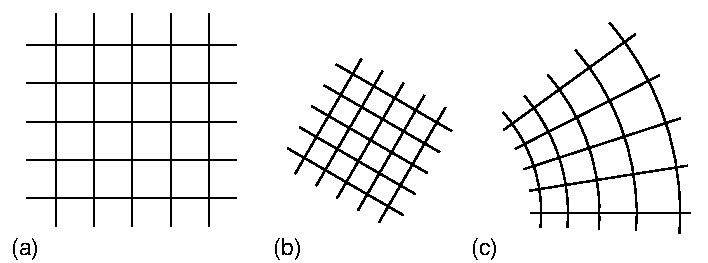
\includegraphics[width=0.8\linewidth]{figures/fig_2_2.pdf}
\caption{(a) 二次元の領域。(b) 特殊な共形変換\hyperref[eq:2.4.9]{(2.4.9)}の作用。(c) より一般的な共形変換の作用。}
\label{fig:2.2}
\end{figure}

\subsubsection*{共形不変性と OPE}

共形不変性は OPE の形、とくにエネルギー運動量テンソルの OPE に強い制約を課す。$T$ と一般の演算子 $\mathcal A$ の OPE を考えよう。$T(z)$ と $\widetilde T(\bar z)$ は挿入の位置を除いて（反）正則なので、対応する係数関数もこの性質をもたなければならない。したがって、$T$ と一般の $\mathcal A$ の OPE は、$z$ の整数べきで、ただし負のべきを含みうる Laurent 展開となる。さらに、すべての特異項は $\mathcal A$ の共形変換によって決まる。これを見るため、特異項の一般的な展開を
\begin{equation}
T(z)\mathcal A(0,0)\sim
\sum_{n=0}^{\infty}\frac1{z^{n+1}}\mathcal A^{(n)}(0,0)
\tag{2.4.11}\label{eq:2.4.11}
\end{equation}
と書き、$\widetilde T$ についても同様に書こう。演算子係数 $\mathcal A^{(n)}$ は、まだ決まっていない。無限小共形変換 $z'=z+\epsilon v(z)$ の下では、$T\mathcal A$ の OPE の $z^{-n-1}$ の項と $v(z)$ の $z^n$ 次の項を掛けたとき、$v(z)T(z)\mathcal A(0,0)$ に単純極が生じる。したがって、\hyperref[eq:2.3.11]{(2.3.11)}の形の Ward 恒等式は、
\begin{equation}
\delta\mathcal A(z,\bar z)
=-\epsilon\sum_{n=0}^\infty\frac1{n!}
\left[\partial^nv(z)\mathcal A^{(n)}(z,\bar z)
+\bar\partial^nv(z)^*\widetilde{\mathcal A}^{(n)}(z,\bar z)\right]
\tag{2.4.12}\label{eq:2.4.12}
\end{equation}
を意味する。よって、演算子 $\mathcal A^{(n)}$ は $\mathcal A$ の共形変換によって決まる。

局所演算子の基底には、一様な変換\hyperref[eq:2.4.9]{(2.4.9)}の下で固有状態となるものをとると便利である。
\begin{equation}
\mathcal A'(z',\bar z')=\zeta^{-h}\bar\zeta^{-\tilde h}\mathcal A(z,\bar z).
\tag{2.4.13}\label{eq:2.4.13}
\end{equation}
$(h,\tilde h)$ は $\mathcal A$ のウェイトと呼ばれる。和 $h+\tilde h$ は $\mathcal A$ の次元であり、スケール変換の下での振る舞いを決める。一方、$h-\tilde h$ はスピンであり、回転の下での振る舞いを決める。微分 $\partial_z$ は $h$ を一つ増やし、微分 $\partial_{\bar z}$ は $\tilde h$ を一つ増やす。変換\hyperref[eq:2.4.13]{(2.4.13)}および並進
$\delta\mathcal A=-\epsilon v^a\partial_a\mathcal A$ に対する Ward 恒等式は、OPE の一部を決める。
\begin{equation}
T(z)\mathcal A(0,0)
=\cdots+\frac h{z^2}\mathcal A(0,0)
+\frac1z\partial\mathcal A(0,0)+\cdots.
\tag{2.4.14}\label{eq:2.4.14}
\end{equation}
$\widetilde T$ についても同様である。

重要な特殊例は、テンソル演算子、あるいは一次場\footnote[3]{場の量子論では通常、基本場（経路積分での積分変数）と、複合的でありうる、より一般的な演算子を区別する。実際には、この区別は主として三次元以上の弱結合の場の理論で有用である。CFT では、とくに異なる場の理論の間に等価関係があるため、ほとんど役に立たない。そこで、任意の局所演算子に対して「場」という語を用いる。}
$\mathcal O$ であり、一般の共形変換はそれに
\begin{equation}
\mathcal O'(z',\bar z')
=(\partial_z z')^{-h}
(\partial_{\bar z}\bar z')^{-\tilde h}\mathcal O(z,\bar z)
\tag{2.4.15}\label{eq:2.4.15}
\end{equation}
と作用する。OPE \hyperref[eq:2.4.11]{(2.4.11)}は
\begin{equation}
T(z)\mathcal O(0,0)
=\frac h{z^2}\mathcal O(0,0)+\frac1z\partial\mathcal O(0,0)+\cdots
\tag{2.4.16}\label{eq:2.4.16}
\end{equation}
に帰着し、一般の OPE \hyperref[eq:2.4.14]{(2.4.14)}にある、より特異な項は存在しない。

再び自由な $X^\mu$ の CFT を例にとると、いくつかの代表的な演算子のウェイトは
\begin{equation}
\left.
\begin{array}{c@{\quad}c@{\qquad}c@{\quad}c}
X^\mu&(0,0)&\partial X^\mu&(1,0)\\
\bar\partial X^\mu&(0,1)&\partial^2X^\mu&(2,0)\\
:e^{ik\cdot X}:&
\displaystyle\left(\frac{\alpha'k^2}4,\frac{\alpha'k^2}4\right)&&
\end{array}
\right\}
\tag{2.4.17}\label{eq:2.4.17}
\end{equation}
である。$\partial^2X^\mu$ を除き、すべてテンソルとして変換する。より一般に、指数関数と微分の一般的な積を掛けたもの
\begin{equation}
:\left(\prod_i\partial^{m_i}X^{\mu_i}\right)
\left(\prod_j\bar\partial^{n_j}X^{\nu_j}\right)e^{ik\cdot X}:
\tag{2.4.18}\label{eq:2.4.18}
\end{equation}
のウェイトは
\begin{equation}
\left(\frac{\alpha'k^2}4+\sum_i m_i,\,
\frac{\alpha'k^2}4+\sum_j n_j\right)
\tag{2.4.19}\label{eq:2.4.19}
\end{equation}
である。

任意の二つの演算子について、一様な並進、スケール変換、回転を OPE の両辺に適用すると、係数関数の $z$ 依存性が完全に決まる。
\begin{equation}
\mathcal A_i(z_1,\bar z_1)\mathcal A_j(z_2,\bar z_2)
=\sum_k z_{12}^{h_k-h_i-h_j}
\bar z_{12}^{\tilde h_k-\tilde h_i-\tilde h_j}
c^k{}_{ij}\mathcal A_k(z_2,\bar z_2).
\tag{2.4.20}\label{eq:2.4.20}
\end{equation}
ここでは、$c^k{}_{ij}$ は定数となっている。関心のあるすべての場合において、OPE \hyperref[eq:2.4.20]{(2.4.20)}の右辺に現れるウェイトは下から有界であるため、演算子積の特異性の次数は有界である。より一般的な共形変換は OPE にさらに制約を課す。それらは、すべての場の OPE を、一次場の OPE によって決定する。このことは第15章で展開する。

正規順序積の共形変換の性質は、一般には、その積の素朴な変換では与えられないことに注意しよう。たとえば、$X^\mu$ の変換則\hyperref[eq:2.4.7]{(2.4.7)}は、指数関数に対して、素朴には
\begin{equation}
\delta e^{ik\cdot X}
=-\epsilon v(z)\partial e^{ik\cdot X}
-\epsilon v(z)^*\bar\partial e^{ik\cdot X}
\qquad\text{（素朴な式）}
\tag{2.4.21}\label{eq:2.4.21}
\end{equation}
を意味し、それをウェイト $(0,0)$ のテンソルにするはずである。この修正は量子効果であり、一点における演算子の積を定義するために必要な繰り込みによる。具体的には、ここでは正規順序記号 $:\ :$ に含まれる減算 $\ln|z_{12}|^2$ が、座標系を明示的に参照しているために現れる。

\subsubsection*{エネルギー運動量テンソルの共形的性質}

エネルギー運動量テンソルとそれ自身の OPE は、式\hyperref[eq:2.2.11]{(2.2.11)}で得られている。
\begin{equation}
\begin{aligned}
T(z)T(0)
&=\frac{\eta^\mu{}_\mu}{2z^4}
-\frac2{\alpha' z^2}:\partial X^\mu(z)\partial X_\mu(0):
+:T(z)T(0):\\
&\sim\frac D{2z^4}+\frac2{z^2}T(0)+\frac1z\partial T(0).
\end{aligned}
\tag{2.4.22}\label{eq:2.4.22}
\end{equation}
$\widetilde T$ についても同様の結果が成り立つ。$T(z)\widetilde T(\bar z')$ の OPE は非特異でなければならない。点が離れているときには $z'$ に関して反正則なので、$(z-z')$ の極はもてない。同様に、点が離れているときには $z$ に関して正則なので、$(\bar z-\bar z')$ の極ももてない。\footnote[4]{特に断らない限り、OPE は点の間隔がゼロでない場合にのみ成り立ち、デルタ関数の可能性は無視している。本書での応用では、後者は問題にならない。デルタ関数を含めることが有用な場合もあるが、一般にその一部は定義に依存するので、注意が必要である。}
正則演算子と反正則演算子の間の任意の OPE についても、同じことが成り立つ。

したがって、$T$ はテンソルではない。OPE \hyperref[eq:2.4.22]{(2.4.22)}が意味する変換則は、
\begin{equation}
\epsilon^{-1}\delta T(z)
=-\frac D{12}\partial_z^3v(z)
-2\partial_zv(z)T(z)-v(z)\partial_zT(z)
\tag{2.4.23}\label{eq:2.4.23}
\end{equation}
である。

一般の CFT では、$T(z)$ は
\begin{equation}
\epsilon^{-1}\delta T(z)
=-\frac c{12}\partial_z^3v(z)
-2\partial_zv(z)T(z)-v(z)\partial_zT(z)
\tag{2.4.24}\label{eq:2.4.24}
\end{equation}
と変換する。$c$ は中心電荷と呼ばれる定数である。一つの自由スカラーの中心電荷は1であり、$D$ 個の自由スカラーでは $D$ である。変換\hyperref[eq:2.4.24]{(2.4.24)}は、$v$ に関して線形で、$TT$ の OPE の対称性と整合し、一様なスケール変換と回転に対する不変性が要求する三つの下付き $z$ 添字をもつ、最も一般的な形である。スケール変換、回転、並進の対称性は、第2項と第3項の係数を決める。さらに、このような二つの変換の交換子を考えると、$\partial_ac=0$ を示すことができる。そして、位置に依存しない演算子は $c$ 数でなければならないというのは、場の量子論の一般的な結果である。\footnote[5]{議論は次のとおりである。$\mathcal A(\sigma)$ は位置に依存しないと仮定し、ほかの任意の局所演算子 $\mathcal B(\sigma')$ との等時刻交換子を考える。局所性により、空間的に離れていれば両者は可換である。$\mathcal A(\sigma)$ は実際には位置に依存しないので、間隔がゼロでも可換である。したがって、$\mathcal A(\sigma)$ はすべての局所演算子と可換であり、$c$ 数でなければならない。}
対応する $TT$ の OPE は
\begin{equation}
T(z)T(0)\sim\frac c{2z^4}+\frac2{z^2}T(0)+\frac1z\partial T(0)
\tag{2.4.25}\label{eq:2.4.25}
\end{equation}
である。変換則\hyperref[eq:2.4.24]{(2.4.24)}の有限の形は
\begin{equation}
(\partial_z z')^2T'(z')=T(z)-\frac c{12}\{z',z\}
\tag{2.4.26}\label{eq:2.4.26}
\end{equation}
である。ここで $\{f,z\}$ は Schwarz 微分
\begin{equation}
\{f,z\}=\frac{2\partial_z^3f\,\partial_zf
-3\partial_z^2f\,\partial_z^2f}
{2\partial_zf\,\partial_zf}
\tag{2.4.27}\label{eq:2.4.27}
\end{equation}
を表す。これは、無限小の形が正しいこと、そして相次ぐ変換の下で正しく合成されることを確認すれば検証できる（したがって、無限小変換を積分できる）。$\widetilde T$ にも対応する形が成り立つが、一般の CFT では、異なる中心電荷 $\tilde c$ をもつ可能性がある。

後で見るように、エネルギー運動量テンソルがテンソルとして振る舞わないことは、いくつかの重要な物理的帰結をもつ。「テンソルでない」とは、共形変換について述べていることを強調しておく。エネルギー運動量テンソルは、座標変換の下では通常のテンソルとしての性質をもつ。

\subsectionlink{自由な共形場理論}\label{sec:2.5}

この節では、自由場の CFT の三つの族、すなわち線形ディラトン理論、$bc$ 理論、$\beta\gamma$ 理論を論じる。$bc$ 理論は、次章で Polyakov 弦のゲージを固定するときに現れるので、最も直接的に関心のあるものである。しかし、いずれも弦理論にさまざまな応用をもつ。

\subsubsection*{線形ディラトン CFT}

この CFT の族は、同じ作用\hyperref[eq:2.1.10]{(2.1.10)}に基づくが、エネルギー運動量テンソルは
\begin{align}
T(z)&=-\frac1{\alpha'}:\partial X^\mu\partial X_\mu:
+V_\mu\partial^2X^\mu,
\tag{2.5.1a}\label{eq:2.5.1a}\\
\widetilde T(\bar z)&=-\frac1{\alpha'}:\bar\partial X^\mu\bar\partial X_\mu:
+V_\mu\bar\partial^2X^\mu
\tag{2.5.1b}\label{eq:2.5.1b}
\end{align}
である。ここで $V_\mu$ は、ある固定された $D$ 元ベクトルである。$TT$ の OPE を計算すると、標準形\hyperref[eq:2.4.25]{(2.4.25)}であることがわかるが、その中心電荷は
\begin{equation}
c=\tilde c=D+6\alpha' V_\mu V^\mu
\tag{2.5.2}\label{eq:2.5.2}
\end{equation}
となる。$TX^\mu$ の OPE と Ward 恒等式\hyperref[eq:2.4.12]{(2.4.12)}は、共形変換
\begin{equation}
\delta X^\mu=-\epsilon v\partial X^\mu
-\epsilon v^*\bar\partial X^\mu
-\frac\epsilon2\alpha' V^\mu\left[\partial v+(\partial v)^*\right]
\tag{2.5.3}\label{eq:2.5.3}
\end{equation}
を意味する。これは、同じ作用の異なる共形対称性である。場 $X^\mu$ はもはやテンソルとしては変換せず、その変分は非斉次な部分をもつ。ちなみに、二次元の質量のない自由スカラーは、驚くほど多くの対称性をもっており、本書で言及する機会のあるものよりもはるかに多い。

エネルギー運動量テンソルは弦理論で特別な役割を果たし、とくに曲がった計量との結合の仕方を教える。したがって、異なる $V^\mu$ の値は異なる CFT とみなすべきである。ベクトル $V^\mu$ は、時空内の一つの方向を選び出す。そのため、この CFT は Lorentz 不変ではなく、当面のわれわれの関心の対象ではない。この線形ディラトン CFT の物理的解釈の一つを3.7節で見て、後にはいくつかの技術的応用で出会うことになる。

自由スカラー CFT の別の変形は、$X^\mu$ のいくつかを周期的にすることである。これは第8章で取り上げる。

\subsubsection*{$bc$ CFT}

第二の CFT の族は、反交換する場 $b,c$ と作用
\begin{equation}
S=\frac1{2\pi}\int d^2z\,b\bar\partial c
\tag{2.5.4}\label{eq:2.5.4}
\end{equation}
をもつ。任意に与えられた定数 $\lambda$ に対して、
\begin{equation}
h_b=\lambda,\qquad h_c=1-\lambda
\tag{2.5.5}\label{eq:2.5.5}
\end{equation}
を満たすウェイト $(h_b,0)$ と $(h_c,0)$ のテンソルとして $b,c$ が変換するとき、これは共形不変である。したがって、別の CFT の族を得る（第10章で学ぶように、これは実は線形ディラトンの族と同じものである）。以前と同じ方法\hyperref[eq:2.1.15]{(2.1.15)}、\hyperref[eq:2.1.18]{(2.1.18)}で得られる演算子の運動方程式は
\begin{align}
\bar\partial c(z)&=\bar\partial b(z)=0,
\tag{2.5.6a}\label{eq:2.5.6a}\\
\bar\partial b(z)c(0)&=2\pi\delta^2(z,\bar z)
\tag{2.5.6b}\label{eq:2.5.6b}
\end{align}
である。$bb$ と $cc$ の OPE は、源のない運動方程式を満たす。正規順序化された $bc$ 積は
\begin{equation}
:b(z_1)c(z_2):=b(z_1)c(z_2)-\frac1{z_{12}}
\tag{2.5.7}\label{eq:2.5.7}
\end{equation}
である。これは、
\begin{equation}
\bar\partial\frac1z=\partial\frac1{\bar z}
=2\pi\delta^2(z,\bar z)
\tag{2.5.8}\label{eq:2.5.8}
\end{equation}
の帰結として、素朴な運動方程式を満たす。この式は、原点を含む領域で積分し、微分を部分積分することで確認できる。場の一般の積の正規順序化は、組合せの面では $X^\mu$ の CFT と同じであり、縮約項または減算項についての和である。$b,c$ は反交換するため、場を交換すると符号が反転することに注意しなければならない。対にする場を、減算\hyperref[eq:2.5.7]{(2.5.7)}で置き換える前に、反交換させて隣り合う位置まで移すべきである。

演算子積は
\begin{equation}
b(z_1)c(z_2)\sim\frac1{z_{12}},\qquad
c(z_1)b(z_2)\sim\frac1{z_{12}}
\tag{2.5.9}\label{eq:2.5.9}
\end{equation}
である。第二の OPE では、反交換によるものと $z_1\leftrightarrow z_2$ によるものの、二つの符号反転が起こっている。ほかの演算子積は非特異である。
\begin{equation}
b(z_1)b(z_2)=O(z_{12}),\qquad
c(z_1)c(z_2)=O(z_{12}).
\tag{2.5.10}\label{eq:2.5.10}
\end{equation}
これらは正則であるだけでなく、反対称性のために零点をもつ。

Noether の定理から、エネルギー運動量テンソル
\begin{align}
T(z)&=:(\partial b)c:-\lambda\partial(:bc:),
\tag{2.5.11a}\label{eq:2.5.11a}\\
\widetilde T(\bar z)&=0
\tag{2.5.11b}\label{eq:2.5.11b}
\end{align}
が得られる。$T$ と $b,c$ の OPE を計算することによっても、\hyperref[eq:2.5.11a]{(2.5.11)}を確認できる。その OPE は、与えられたウェイトをもつ標準的なテンソルの形\hyperref[eq:2.4.16]{(2.4.16)}になる。$TT$ の OPE は標準形\hyperref[eq:2.4.25]{(2.4.25)}であり、
\begin{equation}
c=-3(2\lambda-1)^2+1,\qquad \tilde c=0
\tag{2.5.12}\label{eq:2.5.12}
\end{equation}
である。これは純粋に正則な CFT であり、$c\ne\tilde c$ となる例である。もちろん、対応する反正則な理論
\begin{equation}
S=\frac1{2\pi}\int d^2z\,\tilde b\,\partial\tilde c
\tag{2.5.13}\label{eq:2.5.13}
\end{equation}
もあり、これは上の理論で $z\leftrightarrow\bar z$ としたものと同じである。

$bc$ 理論は、ゴースト数の対称性 $\delta b=-i\epsilon b$、$\delta c=i\epsilon c$ をもつ。対応する Noether カレントは
\begin{equation}
j=-:bc:
\tag{2.5.14}\label{eq:2.5.14}
\end{equation}
である。ここでも成分は別々に正則と反正則であり、後者はゼロである。正則な $bc$ 場と反正則な $bc$ 場の両方がある場合には、それぞれのゴースト数が別々に保存する。

このカレントはテンソルではない。
\begin{equation}
T(z)j(0)\sim\frac{1-2\lambda}{z^3}
+\frac1{z^2}j(0)+\frac1z\partial j(0).
\tag{2.5.15}\label{eq:2.5.15}
\end{equation}
これは変換則
\begin{equation}
\epsilon^{-1}\delta j=-v\partial j-j\partial v
+\frac{2\lambda-1}{2}\partial^2v
\tag{2.5.16}\label{eq:2.5.16}
\end{equation}
を意味し、その有限の形は
\begin{equation}
(\partial_z z')j_{z'}(z')
=j_z(z)+\frac{2\lambda-1}{2}
\frac{\partial_z^2z'}{\partial_z z'}
\tag{2.5.17}\label{eq:2.5.17}
\end{equation}
である。

$b,c$ が等しいウェイトをもつ唯一の場合は $h_b=h_c=\tfrac12$ であり、このとき中心電荷は $c=1$ である。この場合には、$b\to\psi$、$c\to\bar\psi$ という記法をしばしば用いる。この場合、$bc$ CFT は共形不変性を保って二つに分割できる。
\begin{align}
\psi&=2^{-1/2}(\psi_1+i\psi_2),\qquad
\bar\psi=2^{-1/2}(\psi_1-i\psi_2),
\tag{2.5.18a}\label{eq:2.5.18a}\\
S&=\frac1{4\pi}\int d^2z\,
\left(\psi_1\bar\partial\psi_1+\psi_2\bar\partial\psi_2\right),
\tag{2.5.18b}\label{eq:2.5.18b}\\
T&=-\frac12\psi_1\partial\psi_1-\frac12\psi_2\partial\psi_2.
\tag{2.5.18c}\label{eq:2.5.18c}
\end{align}
各 $\psi$ 理論は、中心電荷 $\tfrac12$ をもつ。

$\lambda=2$、ウェイト $(h_b,h_c)=(2,-1)$ の $bc$ 理論は、次章で Polyakov 弦のゲージ固定に伴う Faddeev--Popov ゴーストとして現れる。$\psi$ 理論は、第2巻のより一般的な弦理論に広く現れる。

\subsubsection*{$\beta\gamma$ CFT}

第三の CFT の族は $bc$ 理論とよく似ているが、場は可換である。$\beta$ は $(h_\beta,0)$ テンソル、$\gamma$ は $(h_\gamma,0)$ テンソルであり、
\begin{equation}
h_\beta=\lambda,\qquad h_\gamma=1-\lambda
\tag{2.5.19}\label{eq:2.5.19}
\end{equation}
である。作用は
\begin{equation}
S=\frac1{2\pi}\int d^2z\,\beta\bar\partial\gamma
\tag{2.5.20}\label{eq:2.5.20}
\end{equation}
である。これらの場も、運動方程式
\begin{equation}
\bar\partial\gamma(z)=\bar\partial\beta(z)=0
\tag{2.5.21}\label{eq:2.5.21}
\end{equation}
によって正則となる。運動方程式と演算子積は、標準的な方法で導かれる。統計が変わっているため、演算子積の一部の符号は異なる。
\begin{equation}
\beta(z_1)\gamma(z_2)\sim-\frac1{z_{12}},\qquad
\gamma(z_1)\beta(z_2)\sim\frac1{z_{12}}.
\tag{2.5.22}\label{eq:2.5.22}
\end{equation}
エネルギー運動量テンソルは
\begin{align}
T&=:(\partial\beta)\gamma:-\lambda\partial(:\beta\gamma:),
\tag{2.5.23a}\label{eq:2.5.23a}\\
\widetilde T&=0
\tag{2.5.23b}\label{eq:2.5.23b}
\end{align}
である。中心電荷は、単に符号が逆になる。
\begin{equation}
c=3(2\lambda-1)^2-1,\qquad \tilde c=0.
\tag{2.5.24}\label{eq:2.5.24}
\end{equation}
$\lambda=\tfrac32$、ウェイト $(h_\beta,h_\gamma)=(\tfrac32,-\tfrac12)$ の $\beta\gamma$ 理論は、第10章で超弦のゲージ固定に伴う Faddeev--Popov ゴーストとして現れる。
